\section{Architectural approach description}
\textbf{Model-view-controller} (usually known as \textbf{MVC}) is a software design pattern commonly used for developing user interfaces that divide the related program logic into three interconnected elements.

This design pattern is considered to be universal when it comes to web application.
Because of how it works, most of the webs, in particular it applies well to the idea that an application is accessed in the following way:
\begin{itemize}
  \item The user asks for some resource
  \item Some underlying data is retrieved from somewhere.
  \item A template is then applied to that data in order to show it to the user.
\end{itemize}

This is undeniably the way the web works, most Web MVC frameworks start from the assumption that each user produces relatively few requests asking for big chunks of resources at a time.
This is exactly what the Restaurant POS project requires when the first requirement is Web-based software serving convenience for the users.

The benefits of of using this approach includes: faster development, the ability to provide multiple views, supports asynchronous technique and avoid model collapsing by only one modification.
This is perfect for popular customer-serving web applications, which in this case is our application.

\begin{figure} [H]
    \centering
    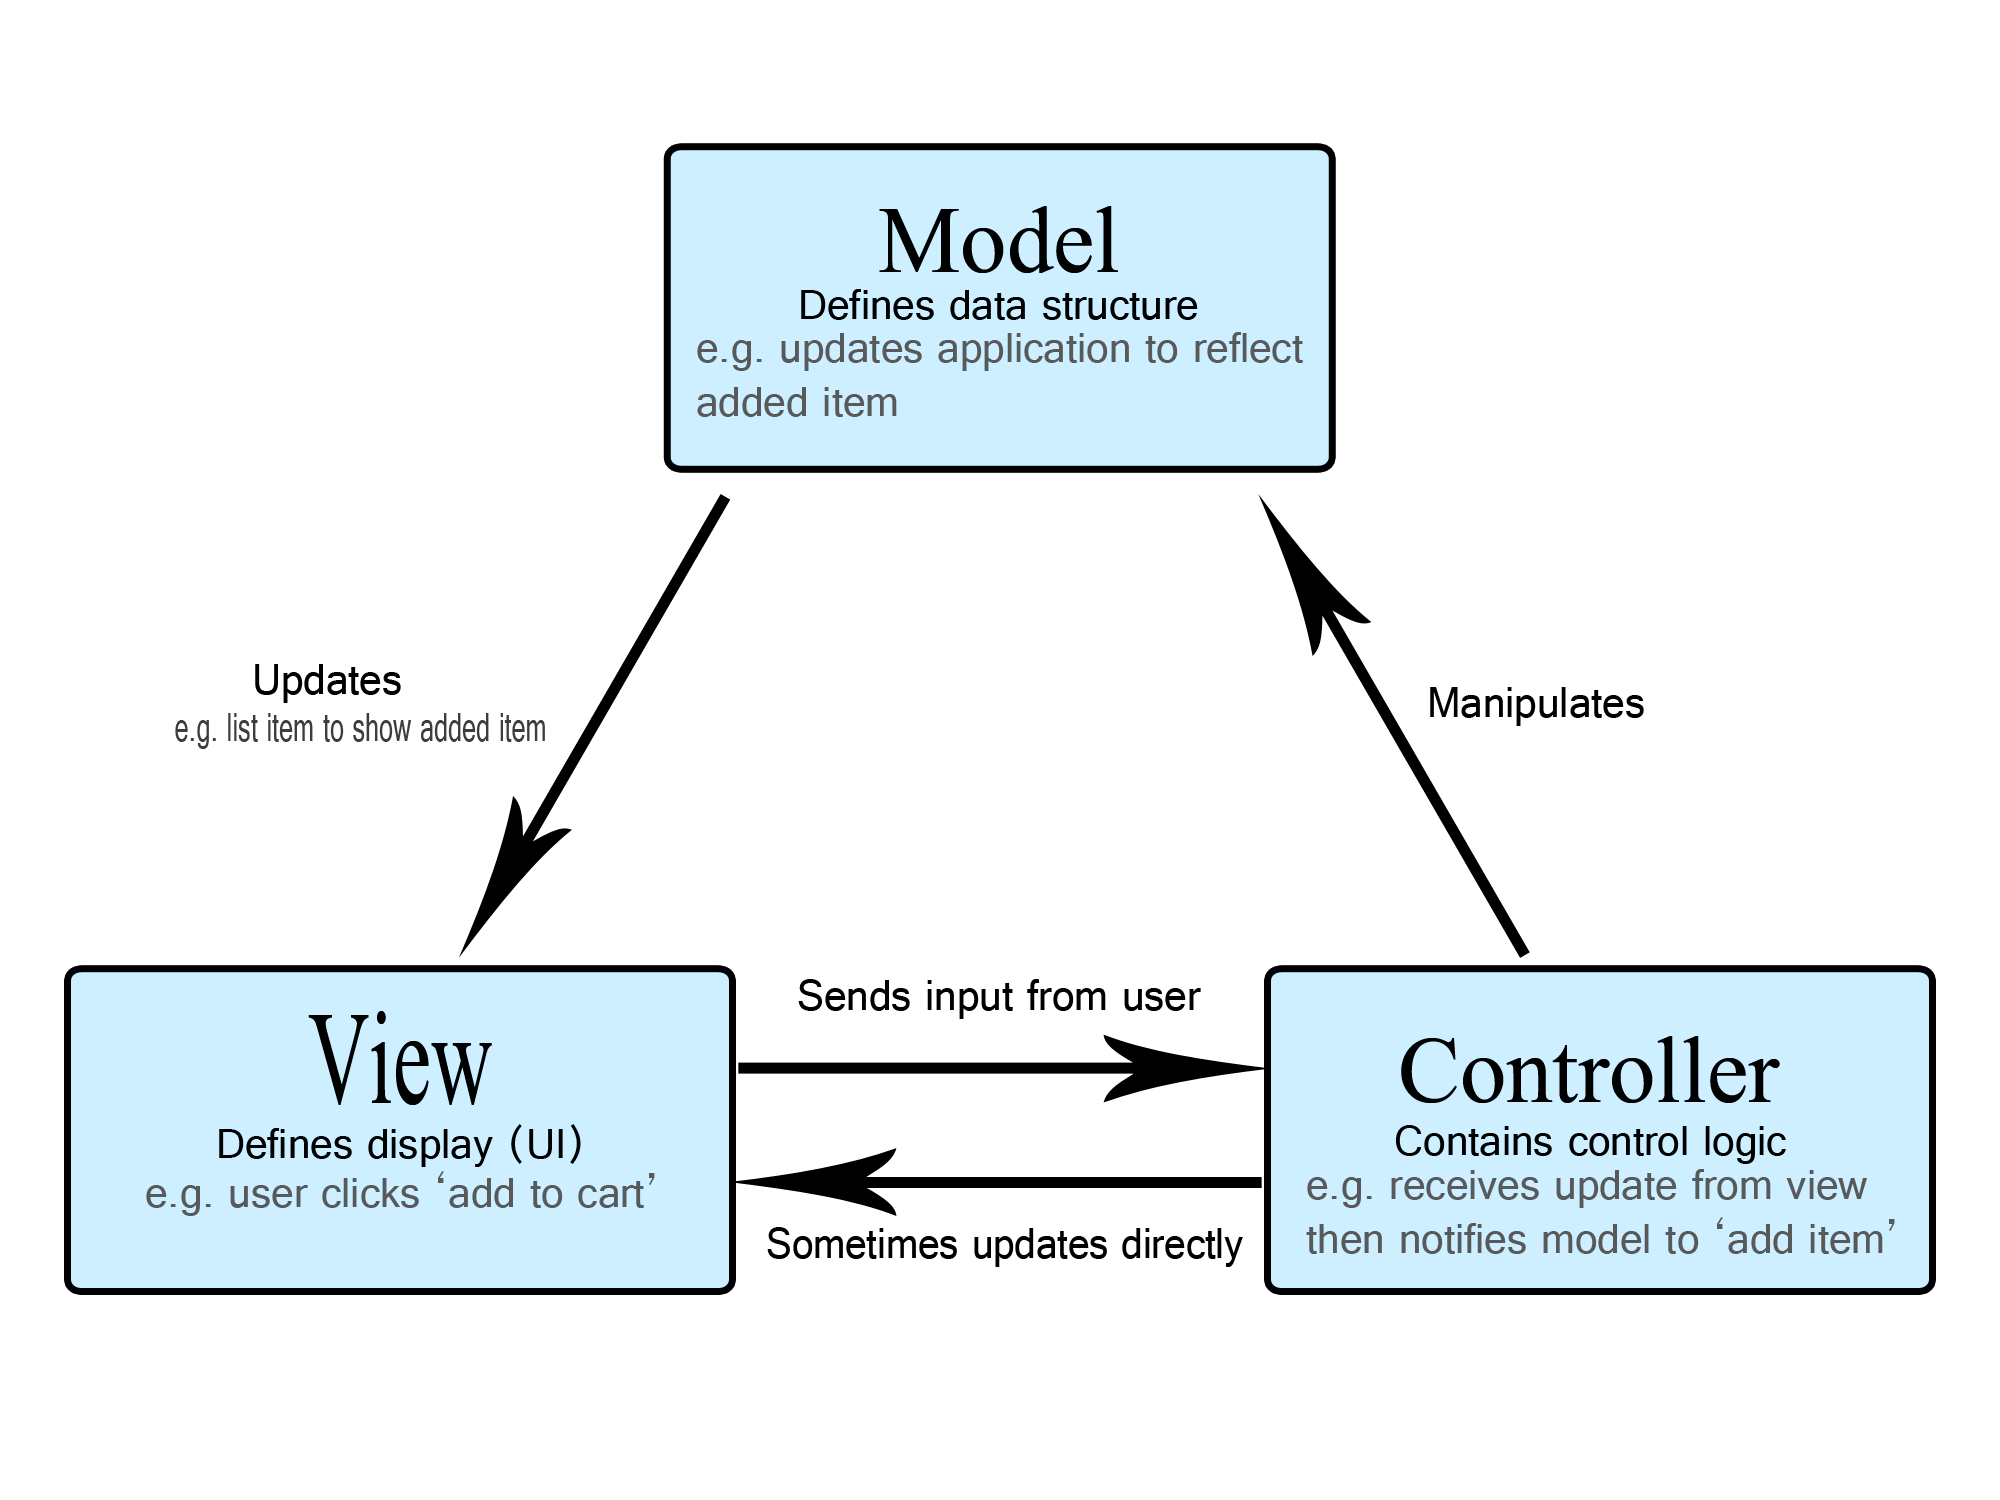
\includegraphics[width=12cm]{assets/t3/model-view-controller.png}
    \caption{MVC diagram}
\end{figure}

\section{Implementation diagram of major functional requirements}

\begin{figure}[H]
  \centering
  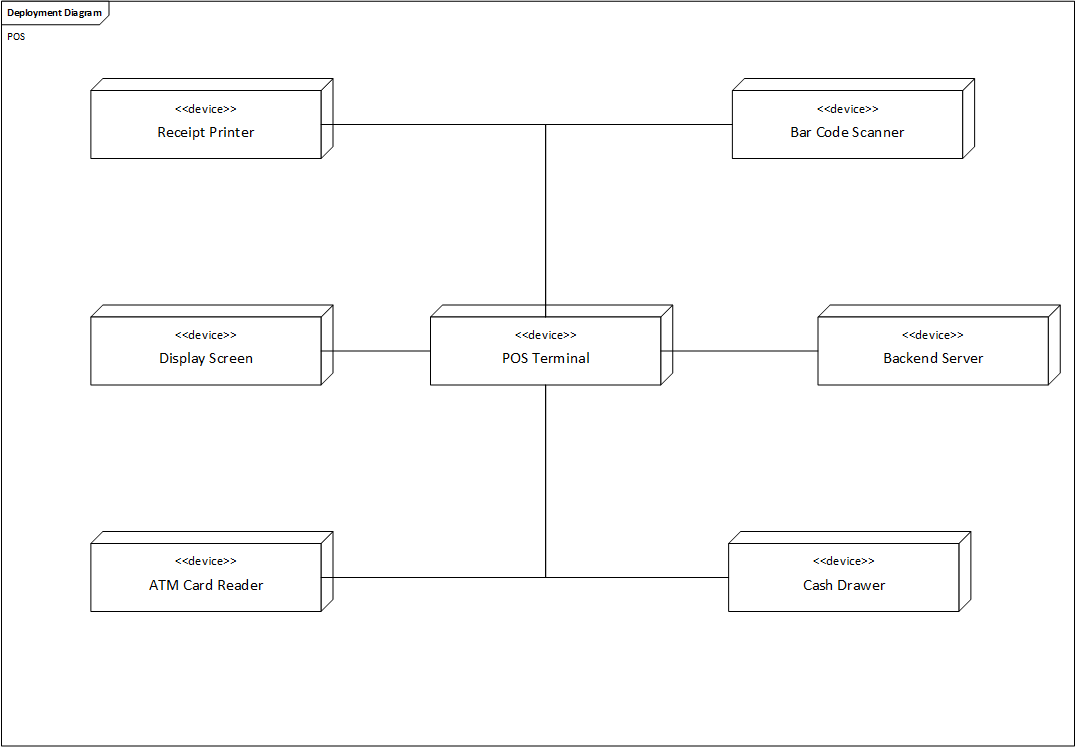
\includegraphics[width=\textwidth]{./assets/t3/deploy.png}
  \caption{Deployment diagram}
\end{figure}
